\documentclass[a4paper,12pt]{article}

%%% Работа с русским языком
\usepackage{cmap}					% поиск в PDF
\usepackage{mathtext} 				% русские буквы в фомулах
\usepackage[T2A]{fontenc}			% кодировка
\usepackage[utf8]{inputenc}			% кодировка исходного текста
\usepackage[english,russian]{babel}	% локализация и переносы

%\usepackage{biblatex} %Imports biblatex package

\usepackage{subcaption}
\usepackage{graphicx}
\usepackage{makecell}
\usepackage{hyperref}
\usepackage[dvipsnames]{xcolor}

%%% Дополнительная работа с математикой
\usepackage{amsfonts,amssymb,amsthm,mathtools} % AMS
\usepackage{amsmath}
\usepackage{icomma} % "Умная" запятая: $0,2$ --- число, $0, 2$ --- перечисление
\usepackage{amsthm}

%% Номера формул
%\mathtoolsset{showonlyrefs=true} % Показывать номера только у тех формул, на которые есть \eqref{} в тексте.

%% Шрифты
\usepackage{euscript}	 % Шрифт Евклид
\usepackage{mathrsfs} % Красивый матшрифт

%% Свои команды
\DeclareMathOperator{\sgn}{\mathop{sgn}}

%% Перенос знаков в формулах (по Львовскому)
\newcommand*{\hm}[1]{#1\nobreak\discretionary{}
	{\hbox{$\mathsurround=0pt #1$}}{}}

%%% Работа с картинками
\usepackage{graphicx}  % Для вставки рисунков
\graphicspath{{images/}{images2/}}  % папки с картинками
\setlength\fboxsep{3pt} % Отступ рамки \fbox{} от рисунка
\setlength\fboxrule{1pt} % Толщина линий рамки \fbox{}
\usepackage{wrapfig} % Обтекание рисунков и таблиц текстом
\usepackage{caption}
\captionsetup{labelsep=period} %. вместо : в рис

%%% Работа с таблицами
\usepackage{array,tabularx,tabulary,booktabs} % Дополнительная работа с таблицами
\usepackage{longtable}  % Длинные таблицы
\usepackage{multirow} % Слияние строк в таблице

\usepackage{extsizes} % Возможность сделать 14-й шрифт
\usepackage{geometry} % Простой способ задавать поля
\geometry{top=25mm}
\geometry{bottom=35mm}
\geometry{left=10mm}
\geometry{right=15mm}

\begin{document}
	
	\begin{titlepage}
		\begin{center}
			
			\vspace{0.5cm}
			\large
			Московский физико-технический институт 
			
			(национальный исследовательский университет)
			\vspace{0.25cm}
			
			Физтех-школа радиотехники и компьютерных технологий \\
			
			Кафедра мультимедийных технологий и телекоммуникаций
			\vfill
			
			\textsc{Практическое задание №2}\\[5mm]
			
			{\LARGE Анализ независимых компонент}
			\bigskip
			
			Назмиев Айрат, 5 курс, группа М01-305
		\end{center}
		\vfill
		
		\newlength{\ML}
		\settowidth{\ML}{«\underline{\hspace{0.7cm}}» \underline{\hspace{2cm}}}
		
		\vfill
		\vfill
		
		\begin{center}
			Москва, 2024 г.
		\end{center}
		
	\end{titlepage}
	
	\section*{Цель работы}
	В данной работе рассматривается анализ независимых компонент (АНК, англ. Independent Component Analysis, ICA) --- метод слепого разделения многомерного сигнала на независимые аддитивные компоненты. Получены аналитические выражения для вычисления энтропии и ее градиента. Проведен ряд вычислительных экспериментов для различного числа смешанных сигналов, также проведен эксперимент с записью на диктофон.
	
	\section*{Введение}
	
	Рассмотрим простейшую модель смешивания сигналов. Пусть имеется $N$ независимых источников сигнала и $M$ сенсоров, для простоты рассмотрим случай $N = M$ (в общем случае необходимо $M \ge N$). Распространяясь в линейной инвариантной во времени среде без памяти, сигналы накладываются друг на друга, поэтому на сенсорах оказываются видны линейные комбинации сигналов с некоторыми неизвестными коэффициентами. Пусть каждый сигнал после дискретизации имеет длительность $T$ отсчетов, тогда можно записать формулу:
	
	\begin{equation}
		\mathbf{X} = \mathbf{A} \mathbf{S},
	\end{equation} 
	где $\mathbf{S} \in \mathbb{R}^{N \times T}$ --- исходные отсчеты сигналов, $\mathbf{X} \in \mathbb{R}^{M \times T} $ ---  отсчеты сигналов, полученные на сенсорах, $\mathbf{A} \in \mathbb{R}^{M \times N} $ "--- матрица смешения (англ. mixing matrix). Заметим, что в данной модели мы также пренебрегаем временем распространения сигнала до каждого из сенсоров. В приведенной модели задачей линейного АНК является нахождения такой матрицы <<размешивания>> (англ. unmixing matrix) $\mathbf{W} \in \mathbb{R}^{N \times M} $, чтобы данные на сенсорах $\mathbf{Y} \in \mathbb{R}^{M \times T}$ представляли собой исходные сигналы:
	
	\begin{equation}
		\mathbf{Y} = \mathbf{W} \mathbf{X}.
	\end{equation}
	
	При условии того, что $\mathbf{A}$ имеет полный ранг, данная задача имеет точное решение (псевдообратная матрица $\mathbf{A}^+$ для прямоугольной или обратная матрица $\mathbf{A}^+=\mathbf{A}^{-1}$ для квадратной). Однако мы считаем, что $\mathbf{A}$ нам неизвестна, более того, в данной модели не рассматривается возможность непосредственной оценки $\mathbf{A}$ (например, с помощью пилотов). В данном случае может быть полезным АНК, который является слепым методом и не требует знания матрицы смешивания.
	
	АНК предполагает, что сигналы в смеси статистически независимы, кроме того, функции распределения (англ. cumulative distribution function, cdf) каждого из сигналов считаются известными. Для простоты компактности изложения предположим, на данный момент, что функции распределения у всех исходных сигналов $\mathbf{S}_i \in \mathbb{C}^T,\, i=\overline{1,\,T}$ одинаковы и равны $F_s$ (в конце будет дано обобщение на случай разных cdf, которое будет необходимо для последнего эксперимента с диктофоном). Применим к $\mathbf{Y}$ функцию распределения, получим $\mathbf{Z} = F_s(\mathbf{Y})\in \mathbb{C}^{M}$. Так, если удастся идеально восстановить исходные сигналы, то есть $\mathbf{Y} = \mathbf{W} \mathbf{A} \mathbf{S} = \mathbf{A}^+ \mathbf{A} \mathbf{S} =  \mathbf{S}$, то получим $F_s(\mathbf{S})$, при этом $F_s(\mathbf{S}) \sim \mathcal{U}([0;\,1]^N)$, здесь использованы интегральное преобразование (универсальность равномерного распределения) и независимость сигналов \cite{casella2002stat}. Обозначим $F_s = g$
	
	Важным свойством многомерного равномерного распределения независимых величин является то, что оно имеет максимальную энтропию среди распределений с компактным носителем \cite{stone2004ica}. Воспользуемся этим свойством для нахождения unmixing matrix $ \mathbf{W} $. Рассмотрим энтропию сигнала после обработки на сенсорах, матрица $\mathbf{Z}$ представляет собой $T$ последовательных реализаций $\mathbf{z}_t,\; t=\overline{1,\,T}$ случайной величины $\mathbf{z}$. Энтропия $\mathbf{z}$ равна:
	
	\begin{equation} \label{eq:EH}
		H(\mathbf{z}) = -\int\limits_{\mathbb{R}^M} f_z(\mathbf{t}) \log(f_z(\mathbf{t})) d\mathbf{t} = 
		 - \mathbb{E}\left[ \log(f_z(\mathbf{t})) \right], 
	\end{equation}
	
	где $f_z$ --- плотность распределения $\mathbf{z}$. Так как мы считаем, что сигналы независимы (после идеального разделения смеси), можно расписать многомерную плотность как произведение одномерныx: $f_z(\mathbf{z}) = \prod_{i=1}^{M}f_z(z_i)$, поэтому $log(f_z(\mathbf{z})) = \sum_{i=1}^{M} \log f_z(z_i)$. Найдем оценку величины энтропии как математическое ожидание собственной информации по выборке $\mathbf{Z}$ (второе равенство в формуле  (\ref{eq:EH})):
	
	\begin{equation} \label{eq:Hsum}
		H(\mathbf{Z}) = -\frac{1}{T} \sum\limits_{t=1}^{T} \log(f_z(\mathbf{z}_t)) = 
						-\frac{1}{T} \sum\limits_{t=1}^{T} \sum\limits_{i=1}^{M} \log(f_z(z_{t,i})).
	\end{equation}
	
	Известно, что $\mathbf{z} = F_s(\mathbf{y}) = g(\mathbf{y}_t)$. Поэтому плотности вероятностей $f_z$ и $ f_y $  случайных величин $ \mathbf{z} $ и $ \mathbf{y} $ связаны соотношением \cite{kelbert2007stat}:
	
	\begin{equation}
		f_z(\mathbf{z}) = \frac{f_y(\mathbf{y})}{\left|\frac{\partial \mathbf{z}}{\partial \mathbf{y}}\right|},
	\end{equation}
	где $\frac{\partial \mathbf{z}}{\partial \mathbf{y}}$ --- матрица Якоби преобразования, а ${\left|\frac{\partial \mathbf{z}}{\partial \mathbf{y}}\right|}$, модуль определителя данной матрицы --- модуль Якобиана преобразования. Так как величины $z_i$ независимы, то матрица Якоби диагональна, получим:
	
	\begin{equation} \label{eq:f_z_g_same}
	f_z(\mathbf{z}) = \frac{f_y(\mathbf{y})}{\prod_{i=1}^{M} g'(y_i)}.
	\end{equation}
	
	Выразим значение $f_y(\mathbf{y})$ через плотность $f_x(\mathbf{y})$. Так как $\mathbf{y} = \mathbf{W} \mathbf{x}$, то $\frac{\partial \mathbf{y}}{\partial \mathbf{x}} = |\det{\mathbf{W}}| = |\mathbf{W}|$. Аналогично (\ref{eq:f_z_g_same}) можем записать:
	
	\begin{equation} \label{eq:f_y}
	f_y(\mathbf{y}) = \frac{f_x(\mathbf{x})}{|\mathbf{W}|}.
	\end{equation}	
	
	Объединяя формулы (\ref{eq:Hsum}, \ref{eq:f_z_g_same}, \ref{eq:f_y}), получаем итоговое выражения для энтропии сигнала:
	
	\begin{equation}
		H(\mathbf{Z}) = \frac{1}{T} \sum\limits_{t=1}^{T} \sum\limits_{i=1}^{M} \log(g'(y_{t,i})) + \log{|\mathbf{W}|} - H(\mathbf{X}),
	\end{equation}
	
	где мы заметили, что последнее слагаемое получилось равным по определению $H(\mathbf{X})$. Так как в модели $H(\mathbf{X})$ не зависит от выбора матрицы $\mathbf{W}$, мы можем убрать его из рассмотрения как постоянное слагаемое в энтропии. Будем рассматривать следующую величину:
	
	\begin{equation} \label{eq:h}
		h_{\mathbf{W}}(\mathbf{Z}) = 
		\frac{1}{T} \sum\limits_{t=1}^{T} \sum\limits_{i=1}^{M} \log(g'(y_{t,i})) + \log{|\mathbf{W}|} = 
		\frac{1}{T} \sum\limits_{t=1}^{T} \sum\limits_{i=1}^{M} \log(g'((\mathbf{W} \mathbf{y})_{t,i})) + \log{|\mathbf{W}|}.
	\end{equation}
	Ниже именно (\ref{eq:h}) будем называть энтропией. Теперь перед нами стоит задача максимизации (\ref{eq:h}), что будет означать, что $g'(y_{t,i})$ распределены равномерно и независимы, это будет означать, что удалось разделить смесь сигналов $\mathbf{X}$ с помощью матрицы $\mathbf{W}_\ast$ и получить исходные сигналы $\mathbf{S}$. Задача АНК ставится следующим образом:
	
	\begin{equation} \label{eq:argmax}
		\mathbf{W}_\ast = \underset{\mathbf{W}}{\arg\max}\; h_{\mathbf{W}}(\mathbf{Z}).
	\end{equation}
	
	Решим данную задачу с использованием градиентного метода. Можно легко показать, что градиент (\ref{eq:h}) по unmixing matrix $\mathbf{W}$ имеет вид \cite{stone2004ica}:
	
	\begin{equation} \label{eq:grad_h_full}
		\frac{\partial h_{\mathbf{W}}}{\partial \mathbf{W}_{i,j}} = 
		\begin{pmatrix}\mathbf{W}^{-\mathsf{T}}\end{pmatrix}_{i,j} + 
		\frac{1}{T} \sum\limits_{t=1}^{T} \sum\limits_{i=1}^{M} \frac{g''(y_{i,t})}{g'(y_{i,t})} x_{j,t}.
	\end{equation}
	
	В приведенной выше формуле (\ref{eq:grad_h_full}) предполагается, что все сигналы в смеси имеют одинаковую функцию вероятности $F_s = g$. Однако как упоминалось выше, данная формула легко обобщается на случай различных cdf $F_{s_i} = g_i$ для каждого из исходных сигналов $s_i$. Повторив те же рассуждения, можно показать, что в этом сценарии выражение для энтропии будет иметь вид:
	
	\begin{equation} \label{eq:grad_h_different}
		\frac{\partial h_{\mathbf{W}}}{\partial \mathbf{W}_{i,j}} = 
		\frac{1}{T} \sum\limits_{t=1}^{T} \sum\limits_{i=1}^{M} \frac{g''_i(y_{i,t})}{g'_i(y_{i,t})} x_{j,t}.
	\end{equation}
	
	Формула именно в таком виде будет использована в последнем эксперименте с записью на диктофоне. Градиентый шаг оптимизации (\ref{eq:argmax}) на итерации $k$ будет иметь вид:
	
	\begin{equation}
		\mathbf{W}_k = \mathbf{W}_{k-1} + \alpha \frac{\partial h_{\mathbf{W}}}{\partial \mathbf{W}},
	\end{equation}
	где $\alpha$ --- коэффициент, отвечающий за величину градиентного шага. В данной работе в качестве функции распределения $g$ используются гиперболический тангенс, смесь распределений Лапласа (приближенно описывает cdf речи человека \cite{rad2006sound}) и нормальное распределение. Все формулы для $g$ и производных приведены в приложениях, здесь укажем формулы для $\tanh$:
	
	\begin{equation}
		g(x) = \tanh(x),\quad g'(x) = 1 - \tanh^2(x) = 1 - g^2(x),\quad  g''(x) = -2 \tanh(x) (1 - \tanh^2(x)) = -2 g(x) g'(x)
	\end{equation}
	
	Выбор гиперболического тангенса связан с тем, что он описывает супер-гауссово распределение (распределение с положительным коэффициентом эксцесса, которое характерно для многих <<нешумовых>> сигналов, например, речи), также для него просто вычисляются производные, не требующие выполнения дополнительных сложных операций, зная только значение самой функции.

	
	\section*{Эксперимент}
	
	В работе было поставлено три основных эксперимента: разделение смеси из двух сигналов, разделение смеси из трех сигналов и белого гауссова шума и эксперимент с записью своего голоса на фоне сильного шума на двухканальный микрофон. Важно заметать, что первые два эксперимента синтетические, данные звуковые дорожки искусственно смешиваются припомощи случайной матрицы $\mathbf{A}$, все сигналы в каждой смеси идеально выровнены друг относительно друга. С третьим экспериментом возникло множество сложностей, связанных с нереалистичностью модели смешения сигнала. Подробнее об этом написано в соответствующем разделе. 
	
	Код, содержащий описание алгоритма с иллюстрациями, проигрыванием аудиодорожек и комментариями, находятся в приложении к отчету, здесь приводятся основные графики и некоторые рассуждения.
	
	\section*{Первый эксперимент}
	
	\begin{figure}[h!]
		\centering
		\begin{subfigure}{0.3\linewidth}
			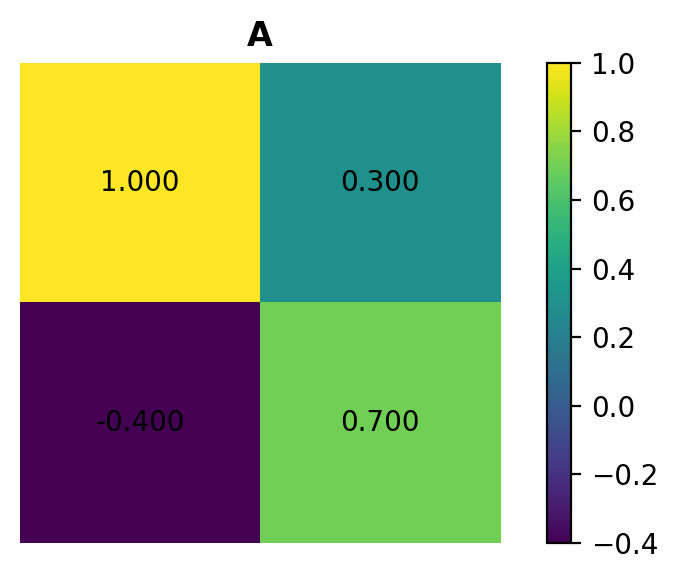
\includegraphics[width=\linewidth]{plots/A1}
		\end{subfigure}
		\begin{subfigure}{0.3\linewidth}
			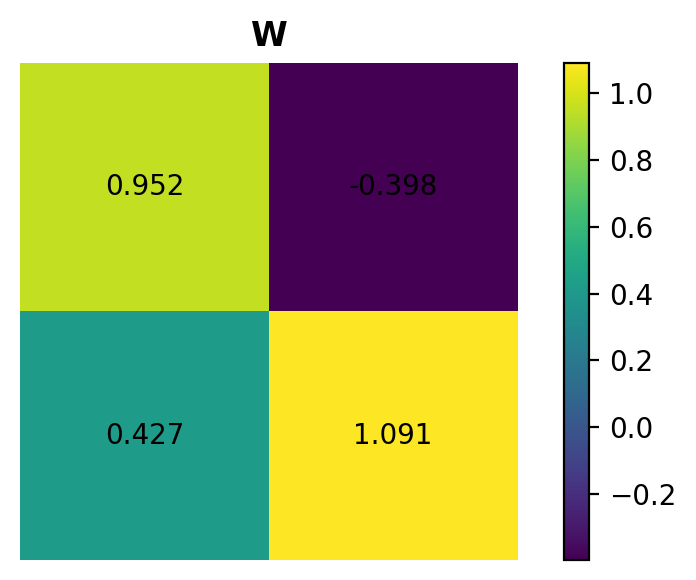
\includegraphics[width=\linewidth]{plots/W1}
		\end{subfigure}
		\begin{subfigure}{0.3\linewidth}
			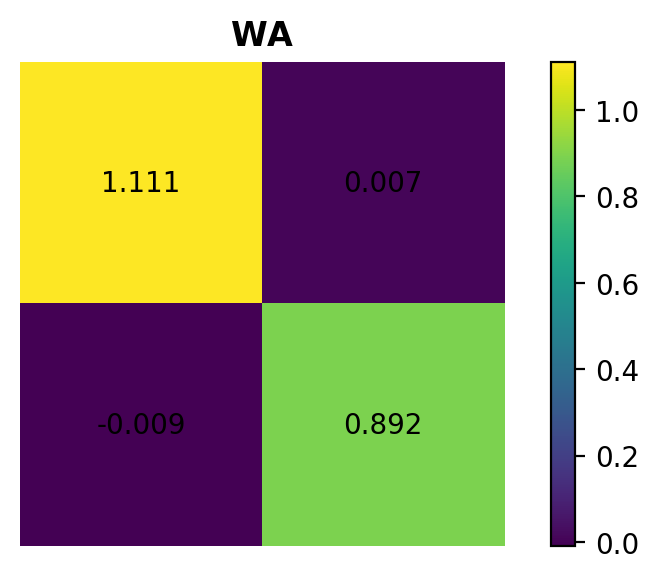
\includegraphics[width=\linewidth]{plots/WA1}
		\end{subfigure}
		
		\caption{Визуализация mixing matrix $\mathbf{A}$, unmixing matrix $\mathbf{W}$ и их композиции $\mathbf{WA}$}
	\end{figure}
	
	\begin{figure}[h!]
		\centering
		\begin{subfigure}{0.3\linewidth}
			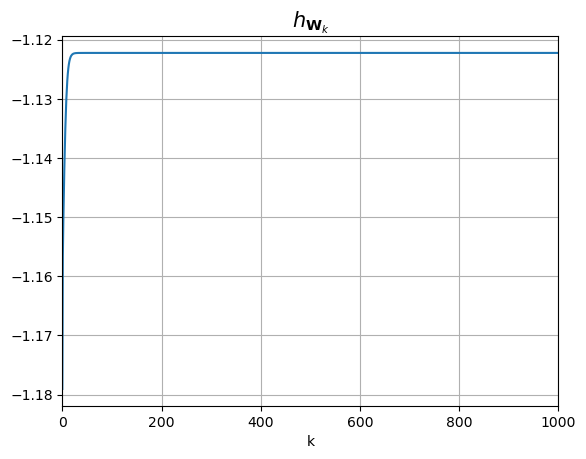
\includegraphics[width=\linewidth]{plots/h1}
		\end{subfigure}
		\begin{subfigure}{0.3\linewidth}
			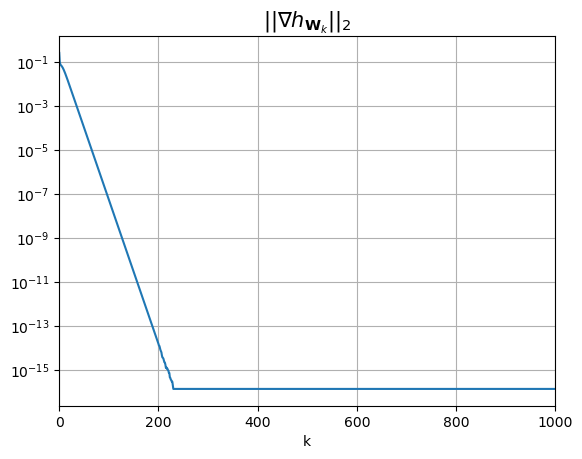
\includegraphics[width=\linewidth]{plots/grad1}
		\end{subfigure}
		\caption{Оптимизация энтропии и изменение второй нормы градиента энтропии}
	\end{figure}
	
	В данном эксперименте использовались две звуковые дорожки ($N=M=2$): пение птицы $\mathbf{s}_1$ и гонг $\mathbf{s}_2$. Рассмотрим mixing matrix $\mathbf{A}$, приведенную на рисунке выше. Можно заметить, что в ходе оптимизации была найдена unmixing matrix $\mathbf{W}$, которая почти идеально разделила сигналы  $\mathbf{X} $ на двух виртуальных сенсорах (микрофонах), так что в композиции матриц $\mathbf{WA}$ дает практически диагональную матрицу. Стоит заметить, что матрица не является единичной, так как АНК не гарантирует выравнивание сигналов по мощности, разделенные сигналы могут получиться произвольно масштабируемыми. Нормировку по уровню сигнала можно сделать уже после отрабатывания алгоритма на полученной оценке $\mathbf{y}_1$ и $\mathbf{y}_2$.
	
	Стоит заметить, что при плохой обусловленности матрицы $\mathbf{A}$ разделить смеси в данной простой линейной модели разделения сигналов не представляется возможным --- обратная матрица будет иметь большие значения элементов, что крайне негативно скажется на процессе оптимизации, или вовсе не существовать (для вырожденной матрицы).
	
	\newpage
	\section*{Второй эксперимент}
	\begin{figure}[h!]
		\centering
		\begin{subfigure}{0.3\linewidth}
			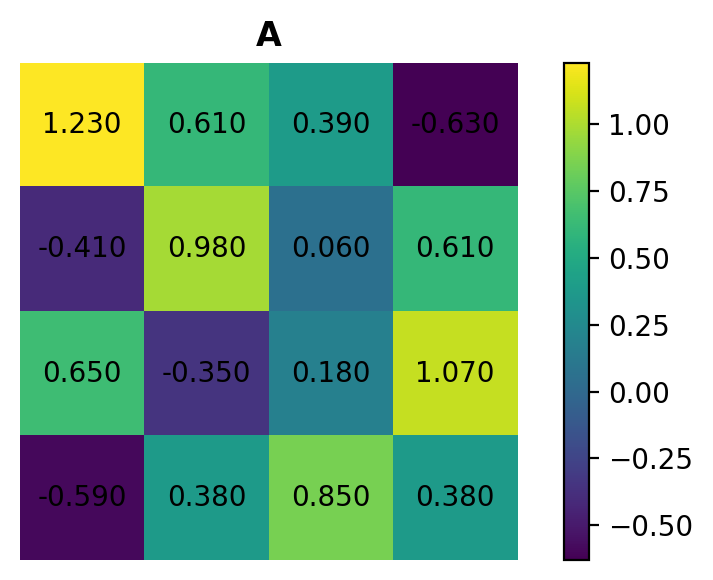
\includegraphics[width=\linewidth]{plots/A2}
		\end{subfigure}
		\begin{subfigure}{0.3\linewidth}
			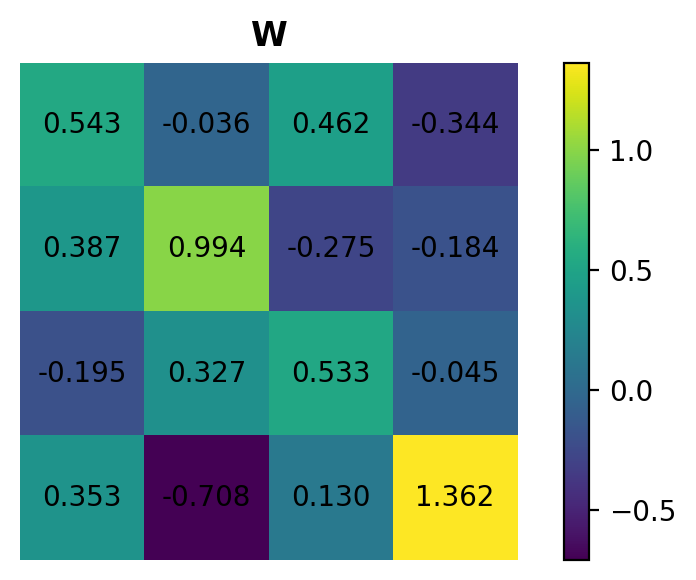
\includegraphics[width=\linewidth]{plots/W2}
		\end{subfigure}
		\begin{subfigure}{0.3\linewidth}
			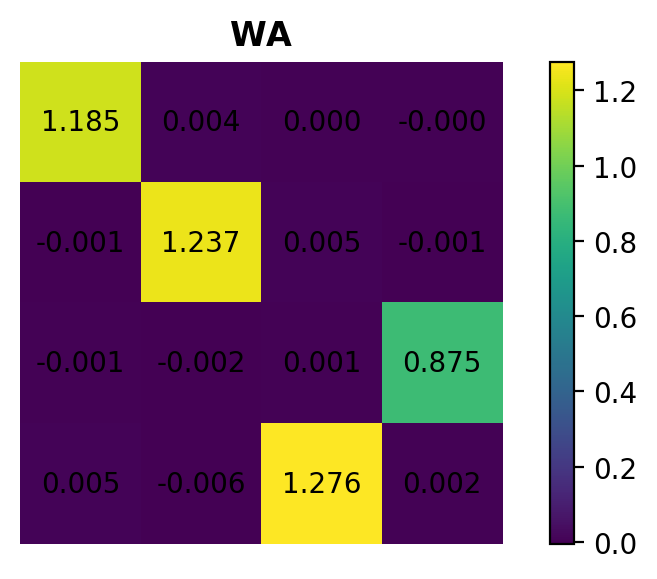
\includegraphics[width=\linewidth]{plots/WA2}
		\end{subfigure}
		
		\caption{Визуализация mixing matrix $\mathbf{A}$, unmixing matrix $\mathbf{W}$ и их композиции $\mathbf{WA}$}
	\end{figure}
	

	
	\begin{figure}[h!]
		\centering
		\begin{subfigure}{0.3\linewidth}
			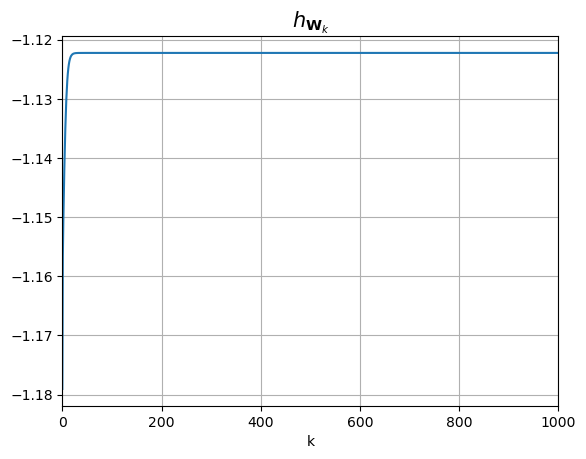
\includegraphics[width=\linewidth]{plots/h1}
		\end{subfigure}
		\begin{subfigure}{0.3\linewidth}
			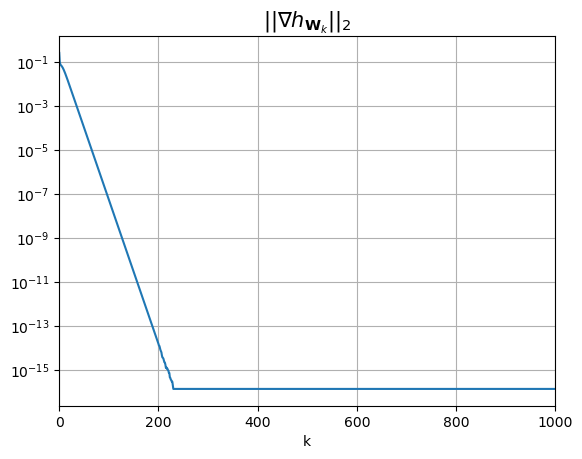
\includegraphics[width=\linewidth]{plots/grad1}
		\end{subfigure}
		\caption{Оптимизация энтропии и изменение второй нормы градиента энтропии}
	\end{figure}
	
	Во втором эксперименте использовались три записи голоса и одна дорожка с белым гауссовым шумом ($N=M=4$). Здесь также удалось полностью разделить сигналы. Однако кроме различий в нормировке уровня сигналов также можно заметить, что третий и четвертый сигнал поменялись местами. Это не проблема, ведь нам требуется просто разделить сигналы, АНК по своей постановке не дает гарантий на сохранение порядка сигналов. Таким образом, при успешной работе алгоритма из смеси будут получены исходные сигналы с точностью до нормировки по мощности и перестановки. Также стоит заметить, что АНК в такой постановке не может устойчивым образом разделить сигналы, содержащие более одной шумовой дорожки, так как любая линейная комбинация, например, двух независимых белых гауссовых случайных процессов также является белым гауссовым случайным процессом. Данный факт может привести к произвольно большим значениями коэффициентов матрицы $\mathbf{W}$.
	
	\newpage
	\section*{Третий эксперимент}
	
	\begin{figure}[h!]
		\centering
		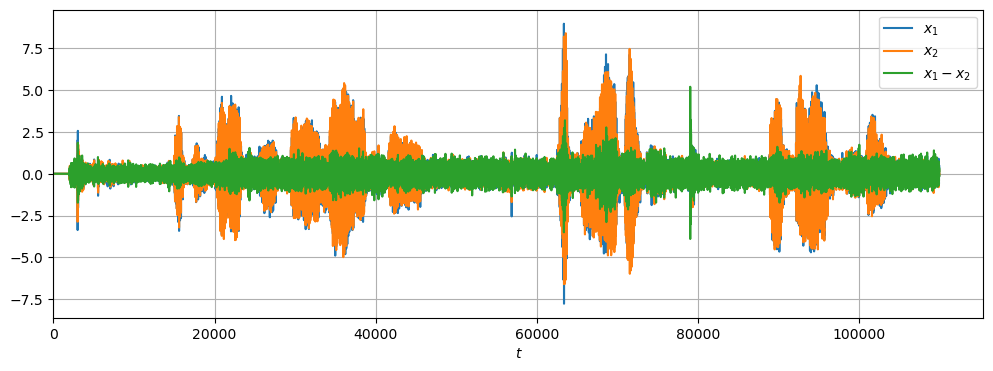
\includegraphics[width=0.6\linewidth]{plots/signal3}
		\caption{Запись сигналов речи и белого гауссова шума на двухканальный микрофон}
	\end{figure}
	
		
	\begin{figure}[h!]
		\centering
		\begin{subfigure}{0.3\linewidth}
			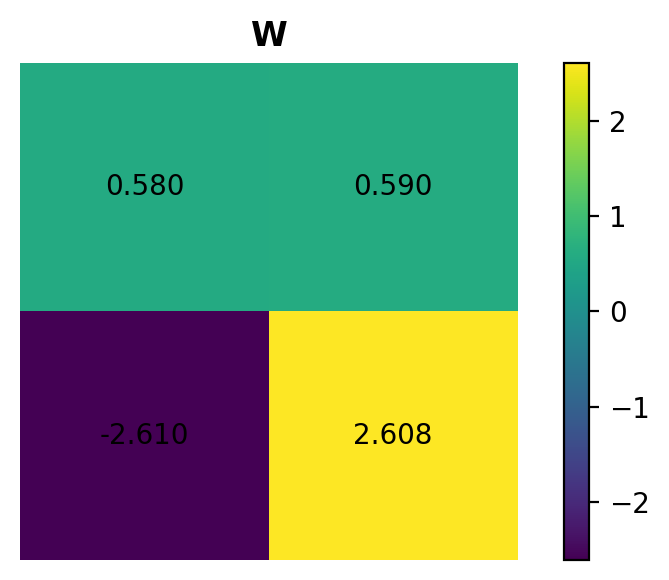
\includegraphics[width=\linewidth]{plots/W3}
		\end{subfigure}
		\begin{subfigure}{0.3\linewidth}
			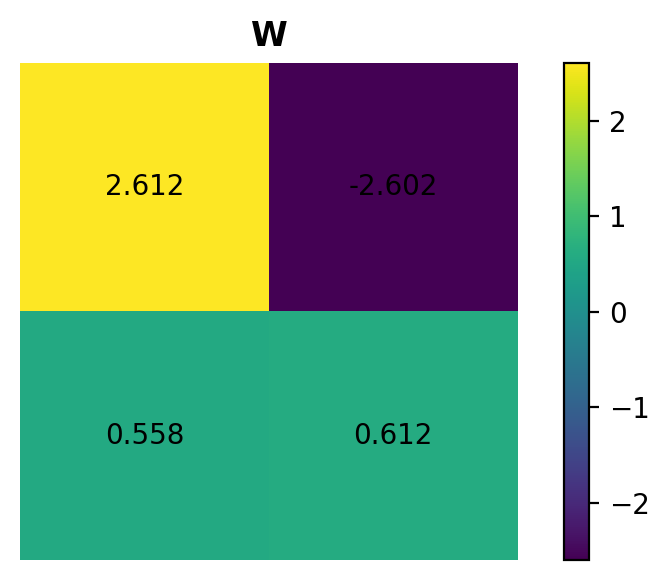
\includegraphics[width=\linewidth]{plots/W3_flip}
		\end{subfigure}
		\caption{Матрицы $\mathbf{W}$ при переставлении местами cdf}
	\end{figure}
	
		\begin{figure}[h!]
		\centering
		\begin{subfigure}{0.3\linewidth}
			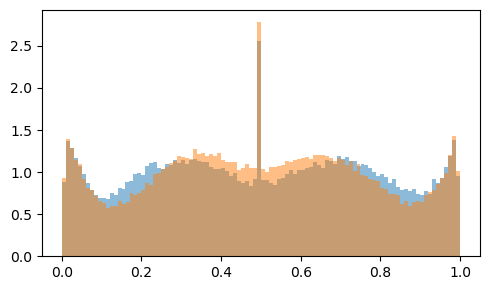
\includegraphics[width=\linewidth]{plots/cdf_matching_1}
		\end{subfigure}
		\begin{subfigure}{0.3\linewidth}
			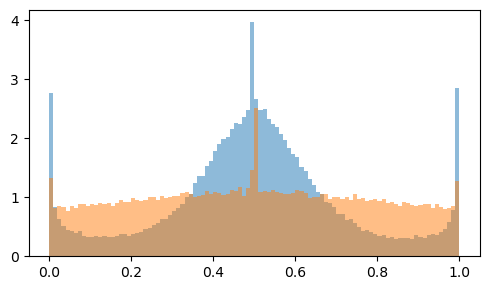
\includegraphics[width=\linewidth]{plots/cdf_matching_2}
		\end{subfigure}
		\caption{Согласование с cdf для двух каналов до (синий) и после оптимизации (оранжевый)}
	\end{figure}
	
	
	\begin{figure}[h!]
		\centering
		\begin{subfigure}{0.3\linewidth}
			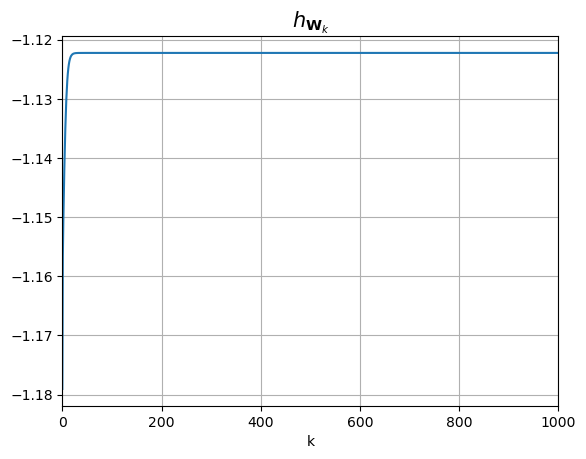
\includegraphics[width=\linewidth]{plots/h1}
		\end{subfigure}
		\begin{subfigure}{0.3\linewidth}
			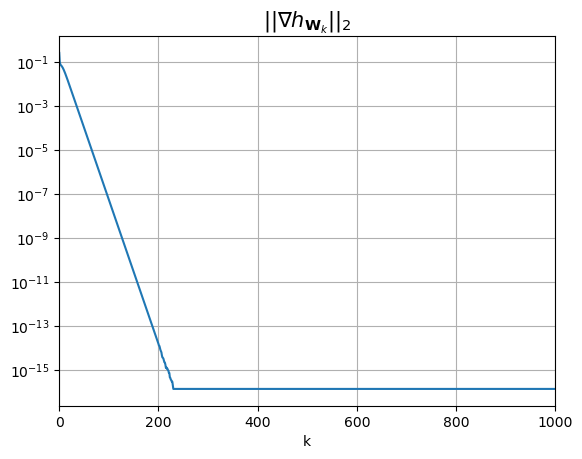
\includegraphics[width=\linewidth]{plots/grad1}
		\end{subfigure}
		\caption{Оптимизация энтропии и изменение второй нормы градиента энтропии}
	\end{figure}
	
	Третий эксперимент производился с записью на диктофон голоса на фоне довольно сильного белого гауссова шума. Рассматриваемая модель смешения сигналов в реальности практически нереализуема (в особенности со звуком): есть довольно длинные импульсные характеристики канала между источниками и приемниками, которые могут значительно отличаться друг от друга, и, кроме того, изменяться во времени. Самая большая проблема заключается в том, что исходные сигналы в каждой из смесей по-разному смещены относительно друг друга, на них по-разному подействовал канал. Так что модель смешения $\mathbf{X} = \mathbf{A} \mathbf{S}$ в общем случае абсолютно не подходит для данного сценария. Однако был рассмотрен крайне выделенный случай, на котором удалось получить интерпретируемый результат.
	
	Для двух сигналов были выбраны различные cdf: смесь распределений Лапласа для голоса и гауссово распределение для белого гауссова шума. Диктофон был поставлен практически ровно посередине между двумя источниками так, чтобы расстояние до каждого из микрофонов для обоих из источников сигналов было близким по величине. Результат оказался довольно простым и, пожалуй, самым естественным в данном сценарии: полусумма для голоса и полуразность для шума, обе величины с некоторым коэффициентом. Интерпретация проста: усредняем шум для отделения дорожки с голосом и дифференцируем, вычитаем для шума. При реальном эксперименте в линейной модели без памяти едва ли можно было ожидать что-то лучше.
	
	Интересно заметить, что при переставлении cdf местами также меняются местами и компоненты смеси: голос и шум согласуются со своими приближенными оценками cdf.
	
	Сигналы также передискретизовывались, фильтровались, чтобы снизить влияние разности задержек и сильнее выделить речь на фоне шума. При необходимости сигналы незначительно выравнивались относительно друг друга. Но без описанных выше строгих условий на постановку эксперимента данные преобразования практически не имеют смысла.
	
	\section*{Выводы}
	
	Метод анализа независимых компонент --- вычислительный метод разделения многомерного сигнала на независимые составляющие. Данный метод является слепым, то есть ему не требуется знать ни исходные сигналы, ни иметь непосредственную информацию о процессе смешивания сигналов. При достаточно слабых, естественных предположениях о независимости сигналов, при наличии некоторой общей модели смешивания есть возможность довольно эффективно разделить или <<доразделить>> сигналы, что активно используется во многих приложениях как самостоятельный, так и как вспомогательный инструмент. АНК находит применение, например, в обработке изображений, звука, данных с датчиков, в беспроводной связи, медицине и других областях, работающих с физическими сигналами \cite{comon2010ica}. 
	
	В данной работе была рассмотрена простейшая линейная модель без памяти, но даже она позволила в синтетических экспериментах справится с сильно перемешанными сигналами. В реальной же задаче разделения звуковых сигналов на диктофоне рассмотренная модель смешивания имеет мало общего с физической реальностью. Существенным, как минимум, является наличие нетривиальной нестационарной импульсной характеристики каналов между источниками и микрофонами, отличие каналов друг от друга. Для решения данной задачи нужно использовать более подходящие, сверточные модели смешивания сигналов, более сложные, возможно, нелинейные модели разделения, рассматривать возможность использования полуслепых методов \cite{comon2010ica}.
	
	
	\clearpage
	\newpage
	\begin{thebibliography}{0}
		\addcontentsline{toc}{section}{\refname}
		\bibitem{stone2004ica} Stone, J. V. Independent Component Analysis: A Tutorial Introduction, 2004
		
		\addcontentsline{toc}{section}{\refname}
		\bibitem{casella2002stat} Casella, G.Statistical Inference, 2002
		
		\addcontentsline{toc}{section}{\refname}
		\bibitem{comon2010ica} Comon, P. and Jutten, C. Handbook of Blind Source Separation: Independent Component Analysis and Applications, 2010
		
		\addcontentsline{toc}{section}{\refname}
		\bibitem{kelbert2007stat} Кельберт М., Сухов Ю. Вероятность и статистика в примерах и задачах. Том I Основные понятия теории вероятностей и математической статистики, 2007		
		
		\addcontentsline{toc}{section}{\refname}
		\bibitem{rad2006sound} Радзишевский, А. Основы аналогового и цифрового звука, 2006		
		
		
	\end{thebibliography}
	
	
\end{document}